
\section{AXOL1TL and TOPO model names}

This document is a description for the naming convetion of AXOL1TL and TOPO model names.

With the release of utm version 0.12, the possibility of setting cuts for different models of Axol1tl and Topological triggers is available.
To prevent changes in utm and TME, we created a structure which is open for upcoming new models without touching utm and TME!\\
The uGT tool "VHDL Producer" and the uGT firmware (VHDL) code depend on the AXOL1TL and TOPO model names. Therefore a convention is necessary.\\
A list of valid AXOL1TL and TOPO model names will be provided on a web page (an example is available \url{https://globaltrigger.web.cern.ch/upgrade/tme/models}).

\subsection{Implementation in Trigger Menu Editor (TME)}

In TME "cut editor" a link to valid model names is available for L1Menu developers to set model names, see Figure \ref{fig:tme_model_cut} for TMODEL (Topological model),
similar for AMODEL (Axol1tl model).

\begin{figure}[htb]
\centering
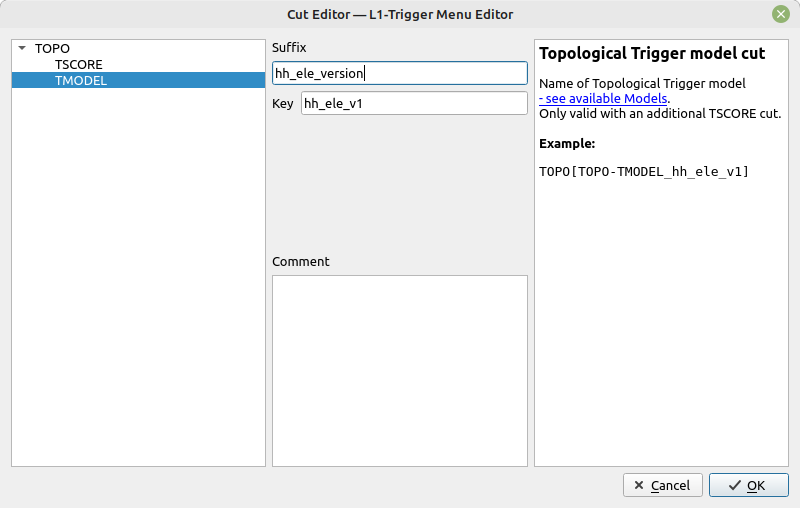
\includegraphics[width=15cm]{figures/tme_model_cut}
\caption{TME cut editor TMODEL}
\label{fig:tme_model_cut}
\end{figure}

\subsection{Implementation in uGT firmware}

The uGT firmware will provide subdirectories for VHDL files of every available model.\\
According to the model names listed in \url{https://globaltrigger.web.cern.ch/upgrade/tme/models}, we created a subdirectory structure as follows:

../
